\chapter{Fundamentals of Retrieval-Augmented Generation}
\label{chap:fundamentals_rag}

Retrieval-Augmented Generation (RAG) is an architectural pattern for LLM-based systems that combines a retrieval component with a generative model. This approach enhances the model's knowledge with external, up-to-date information, addressing common limitations like knowledge cutoffs and hallucination \autocite{lewis2020retrieval, gao2024retrievalaugmented}. This chapter lays the groundwork by explaining the core mechanics of RAG, its main challenges, and the role of its key components.

\section{How it Works}
The foundational RAG architecture, often referred to as \textbf{Naive RAG} \autocite{gao2024retrievalaugmented}, operates in two main stages: retrieval and generation, as originally proposed by Lewis et al. (2020) \autocite{lewis2020retrieval}. This paradigm was significantly influenced by earlier and parallel developments in dense retrieval and knowledge-augmented language models, such as Dense Passage Retrieval (DPR) by Karpukhin et al. (2020) \autocite{karpukhin2020dense} and REALM (Retrieval-Augmented Language Model) by Guu et al. (2020) \autocite{guu2020realm}, which laid crucial groundwork for effectively integrating external knowledge. The process begins when a user submits a query. Instead of directly feeding the query to the LLM, the RAG pipeline intercepts it and first interacts with an external knowledge base.

\begin{enumerate}
    \item \textbf{Retrieval Stage:} The primary objective of this stage is to efficiently identify and extract the most relevant information from a vast external knowledge base that can help answer the user's query. The user's query is converted into a numerical representation, or \textit{embedding}, using a text embedding model. This query embedding is then used to search a pre-indexed collection of documents. The goal is to find and retrieve chunks of text that are semantically similar to the query. This retrieval is typically performed using a vector database, which is optimized for high-speed similarity searches over large datasets of embeddings. The output of this stage is a set of relevant text chunks, often referred to as the \textit{context}.

    
    \item \textbf{Generation Stage:} In this stage, the Large Language Model (LLM) acts as a sophisticated text synthesizer. The goal of this stage is to produce a coherent and factually accurate response by leveraging the retrieved information, a process often referred to as knowledge-grounded generation \autocite{yu2022survey}. The retrieved context is then combined with the original query into a structured prompt. This augmented prompt is fed to the LLM. By providing this explicit, relevant information, the LLM is guided to generate a response that is not only contextually appropriate but also grounded in the facts contained within the retrieved documents, minimizing reliance on its internal, potentially outdated or hallucinated, knowledge. This process significantly enhances the accuracy and factuality of the output.
\end{enumerate}

\begin{figure}[!htbp]
    \centering
    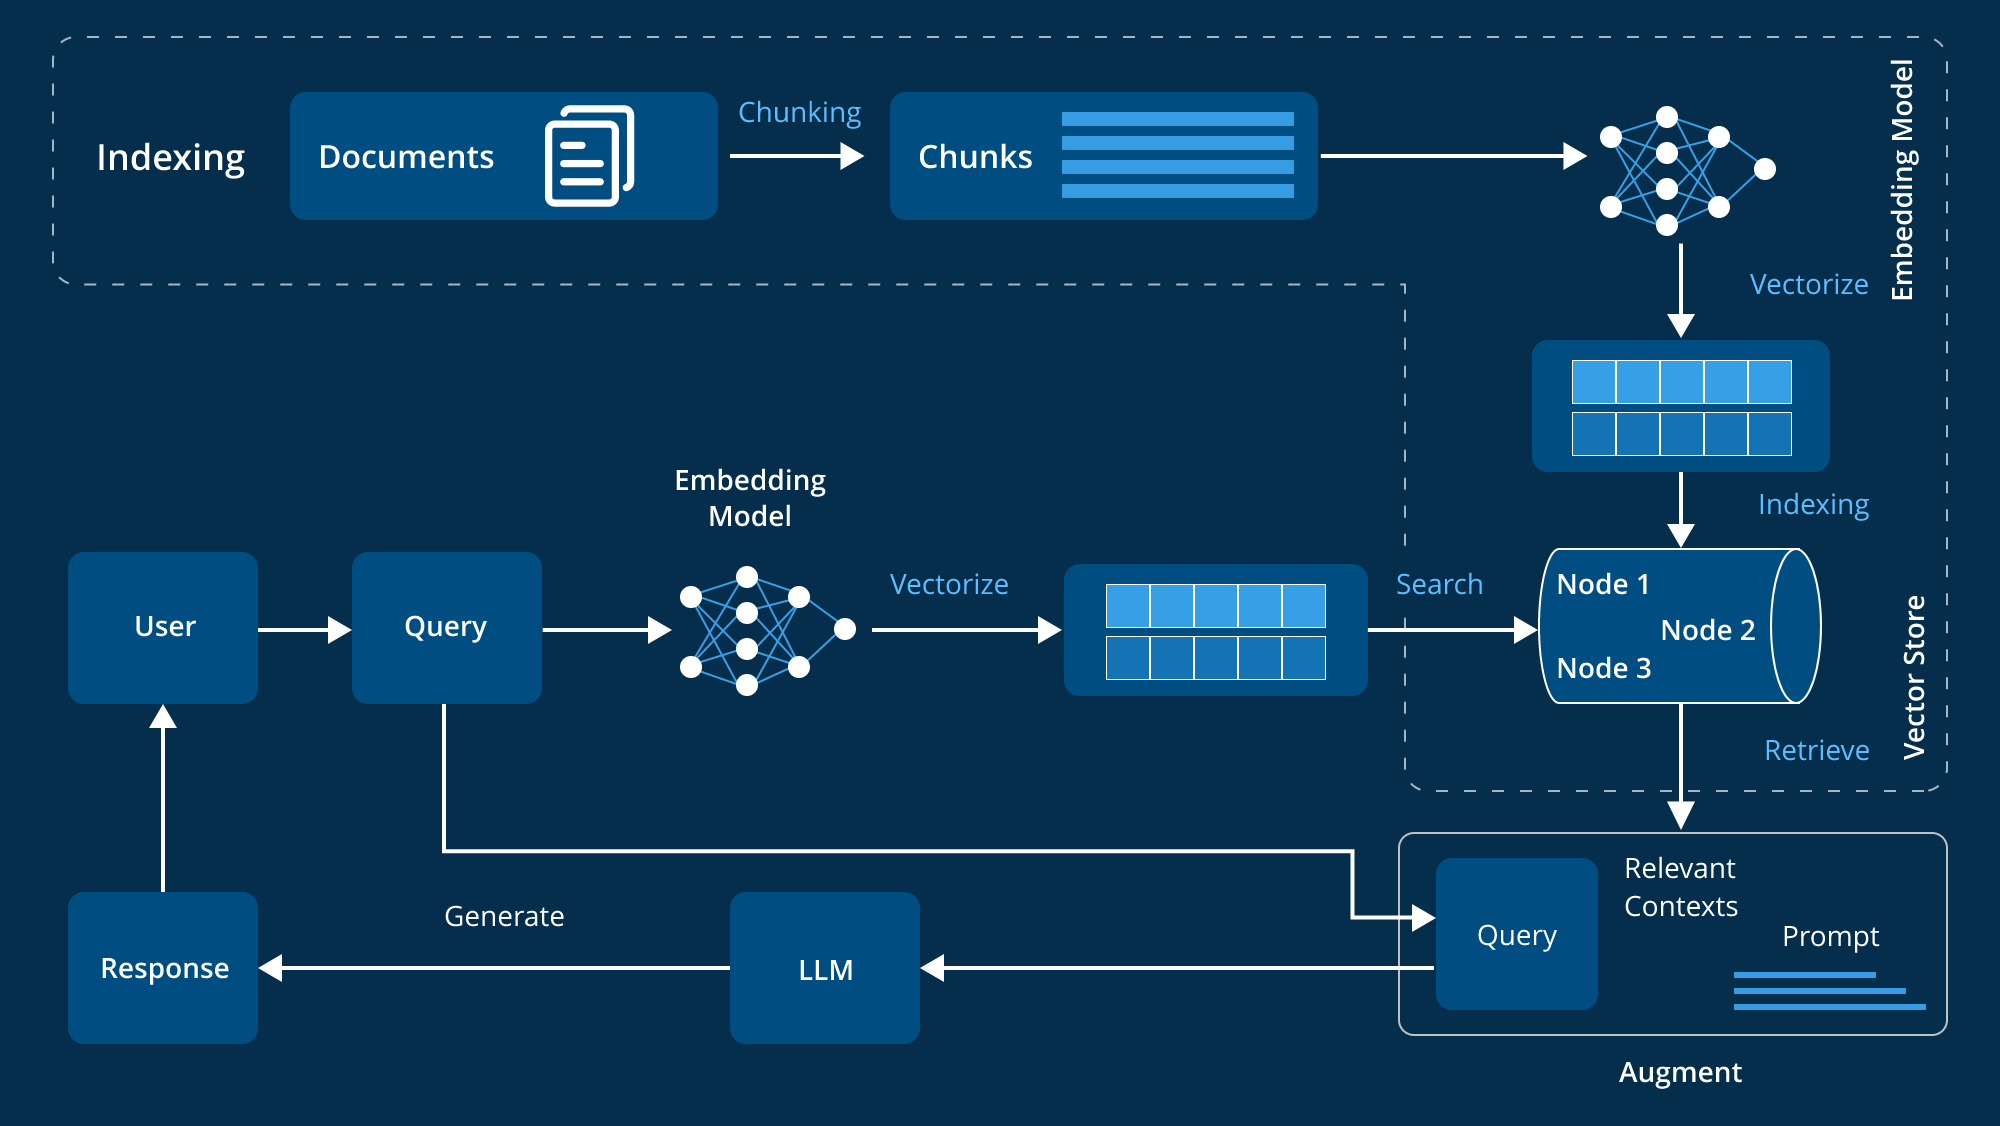
\includegraphics[width=0.9\textwidth]{images/chapter2/rag_architecture_2.png}
    \caption{High-level architecture of a Retrieval-Augmented Generation system.}
    \label{fig:rag_architecture}
\end{figure}

\section{Main Challenges}
The apparent simplicity of the Naive RAG pipeline belies several complex challenges that must be addressed to build a robust and effective system \autocite{gao2024retrievalaugmented}.

\subsection{Ensuring Content Relevance}
The quality of the generated output is fundamentally dependent on the quality of the retrieved context. If the retriever fetches irrelevant or low-quality documents, the LLM may ignore them or, worse, incorporate incorrect information into its response. A key challenge is the \textit{lost in the middle problem}, where LLMs tend to overlook relevant information if it is buried among less relevant chunks in the context window \autocite{liu2023lost}. This phenomenon underscores the need for retrieval systems that not only find relevant documents but also rank them effectively.

\subsection{Optimizing Retrieval vs. Generation Trade-offs}
There is an inherent trade-off between the speed and comprehensiveness of the retrieval step. Retrieving more documents might increase the chance of finding the correct information but also increases the computational load and the risk of introducing noise. The length of the context that can be passed to the LLM is also limited by its context window size. As highlighted by Gao et al. (2024) \autocite{gao2024retrievalaugmented}, optimizing the selection of the most relevant document chunks from the initial similarity search is a key challenge. Techniques like re-ranking retrieved results, which will be explored later in this thesis, are designed to address this trade-off.

\subsection{Handling Noisy or Conflicting Information}
Real-world data is often messy. The retrieved context may contain conflicting facts or irrelevant details. The RAG system must be resilient to such noise, and the LLM must be capable of synthesizing information from multiple sources, identifying contradictions, and prioritizing the most reliable data. Advanced RAG architectures, such as those employing query transformations or reranking, are designed to tackle this issue \autocite{gao2024retrievalaugmented, rag_fusion_2024}.

\subsection{Seamless Integration and Synthesis}
The LLM must be able to seamlessly weave the retrieved information into a coherent and natural-sounding response. This requires not just extracting facts but understanding the nuances of the context and integrating them into a cohesive narrative that directly answers the user's query. The fluency and relevance of the final output are direct measures of the RAG system's success.

\section{Vector Databases and Similarity Search}
The concept of representing text as vectors in a multi-dimensional space for similarity comparison, foundational to modern vector databases, was pioneered by the Vector Space Model (VSM) in 1975 \autocite{salton1975vector}. Vector databases are a cornerstone of modern RAG systems, serving as the indexed knowledge base. They work by storing text data as high-dimensional vectors known as \textit{embeddings}. When a query is received, it is also converted into an embedding, and the database searches for the vectors in its index that are closest to the query vector.



\subsection{Measuring Similarity}
The most common way to measure the distance between two vectors in the context of RAG is \textbf{cosine similarity}, which measures the cosine of the angle between them. For two vectors, A and B, the cosine similarity is calculated as:
\begin{equation}
\text{Cosine Similarity} = \frac{A \cdot B}{\|A\| \|B\|}
\end{equation}
Where \(A \cdot B\) is the dot product of the two vectors, and \(\|A\|\) and \(\|B\|\) are their magnitudes. The result ranges from -1 (exactly opposite) to 1 (exactly the same).
Another common metric is \textbf{Euclidean distance}, which is the straight-line distance between two points in the vector space:
\begin{equation}
\text{Euclidean Distance} = \sqrt{\sum_{i=1}^{n} (A_i - B_i)^2}
\end{equation}

\subsection{The Advantage of Normalized Vectors}
For efficiency, it is a common practice to \textbf{normalize} the vectors before storing them in the database. A normalized vector has a magnitude (or L2 norm) of 1. The magnitude of a vector \(A = [a_1, a_2, \ldots, a_n]\) is computed as:

\begin{equation}
\|A\| = \sqrt{a_1^2 + a_2^2 + \cdots + a_n^2}
\end{equation}

When vectors are normalized, the denominator in the cosine similarity formula (\(\|A\| \|B\|\)) becomes 1. Therefore, the cosine similarity calculation simplifies to just the \textbf{dot product} of the vectors, which is computationally much cheaper:

\begin{equation}
\text{Cosine Similarity (normalized)} = A \cdot B
\end{equation}

This optimization avoids the expensive square root operations needed to calculate the vector magnitudes, allowing for significantly faster similarity searches, which is critical for real-time RAG applications.


\subsection{Indexing for Efficient Search}
To avoid a brute-force search, vector databases use specialized indexing algorithms for Approximate Nearest Neighbor (ANN) search. These algorithms, such as Hierarchical Navigable Small World (HNSW) \autocite{hnsw_malkov_2018} and Inverted File (IVF) \autocite{ivf_zobel}, enable efficient retrieval of the top-k most similar vectors without having to compare the query vector to every single vector in the database. This is crucial for achieving low-latency responses in large-scale RAG systems.

\section{Mitigating Hallucinations}
One of the most significant benefits of RAG is its ability to mitigate LLM hallucinations. By providing factual, verifiable context directly within the prompt, RAG grounds the model's response in reality. The LLM is instructed to formulate its answer based on the provided text, reducing its reliance on its internal, parametric knowledge, which may be outdated or incorrect.

However, RAG is not a perfect solution. Hallucinations in RAG systems can primarily stem from two sources: retrieval failure (e.g., providing irrelevant or inaccurate context) and generation deficiency (e.g., the LLM misinterpreting or ignoring the provided context). If the retrieved context is of poor quality, contains subtle inaccuracies, or is itself misleading, the LLM may still generate a flawed response. Therefore, the quality of the retrieval process is paramount. A well-tuned retriever that provides accurate and relevant context is the first and most critical line of defense against hallucinations in a RAG system \autocite{gao2024retrievalaugmented}.